%\documentclass[aps,prb,onecolumn,nofootinbib]{revtex4}  
\documentclass[12pt,a4paper]{article}
\usepackage[margin=1in]{geometry}  % set the margins to 1in on all sides
%\usepackage{jheppub}
\usepackage{amsmath,amsfonts,amssymb,latexsym,dsfont}
\usepackage{hhline}
\usepackage{graphicx}
\usepackage[arrow,matrix]{xy}
\usepackage{tikz}
\usepackage{tikz-cd}
\definecolor{hanpurple}{rgb}{0.32, 0.09, 0.98}

\usepackage[numbers]{natbib}
\usepackage[colorlinks]{hyperref}
\hypersetup{linkcolor={hanpurple}}





\usetikzlibrary{positioning,arrows}
\usetikzlibrary{decorations.pathmorphing}
\usetikzlibrary{decorations.markings}
\newcommand{\tp}{\otimes}
\newcommand{\ra}{\rightarrow}
\newcommand{\unit}{\mathbf{1}}
\newcommand{\zz}{\mathbb{Z}}
\newcommand{\mce}{\mathcal{E}}
\newcommand{\cc}{\mathbb{C}}
\newcommand{\rr}{\mathbb{R}}
\newcommand{\mcr}{\mathcal{R}}
\newcommand{\mcz}{\mathcal{Z}}
\newcommand{\mca}{\mathcal{A}}
\newcommand{\mcd}{\mathcal{D}}
\newcommand{\mcg}{\mathcal{G}}
\newcommand{\mct}{\mathcal{T}}
\newcommand{\ul}{\underline}
\newcommand{\Mod}{\text{Mod}}
\newcommand{\Aut}{\text{Aut}}
\newcommand{\ulmcc}{\underline{\mathcal{C}}}
\newcommand{\zt}{\mathbb{Z}_2}
\newcommand{\oeo}{\text{others = 1}}
\newcommand\be            {\begin{equation}}
\newcommand\ee            {\end{equation}}
\newcommand\ba            {\begin{aligned}}
\newcommand\ea            {\end{aligned}}
\newcommand{\mcf}{\mathcal{F}}
\newcommand{\spinz}{\text{\sffamily{Z}}}
\newcommand{\spinx}{\text{\sffamily{X}}}
\newcommand{\mcl}{\mathcal{L}}
\newcommand{\mcc}{\mathcal{C}}
\newcommand{\mco}{\mathcal{O}}
\newcommand{\mcm}{\mathcal{M}}
\newcommand{\zc}{\mathcal{Z}(\mathcal{C})}
\newcommand{\id}{\text{id}}
\newcommand{\Hom}{\text{Hom}}
\newcommand{\End}{\text{End}}
\newcommand{\Tor}{\text{Tor}}
\newcommand{\Ext}{\text{Ext}}
\newcommand{\p}{\partial}
\newcommand{\wt}{\widetilde}
\usepackage{verbatim}
\newcommand{\cl}{\mathbb{C}\ell}
\newcommand{\vect}{\text{Vec}}
\newcommand{\svect}{\text{sVec}}
\newtheorem{thm}{Theorem}
\newtheorem{cor}{Corollary}
\newtheorem{lemma}{Lemma}
\newtheorem{prop}{Proposition}
\newtheorem{problem}{Problem}
\newtheorem{defn}{Definition}
\newtheorem{question}{Question}
\newcommand{\fube}{\textbf{Fube}}
\newcommand{\tube}{\textbf{Tube}}
\newcommand{\fld}{\mathcal{F}}

\newcommand{\bra}[1]{\ensuremath{\left\langle#1\right|}}
\newcommand{\ket}[1]{\ensuremath{\left|#1\right\rangle}}

\definecolor{ao(english)}{rgb}{0.0, 0.5, 0.0}
\definecolor{americanrose}{rgb}{1.0, 0.01, 0.24}
\definecolor{amber(sae/ece)}{rgb}{1.0, 0.49, 0.0}

\newcommand{\dave}[1]{{\color{ao(english)}\footnotesize{(DA) #1}}}
\newcommand{\remove}[1]{{\color{amber(sae/ece)}\footnotesize{(RM?) #1}}}

%a purple that looks different from red. EL: nice! I like the name
\definecolor{amethyst}{rgb}{0.6, 0.4, 0.8}
\newcommand{\ethan}[1]{{\color{amethyst}\footnotesize{(EL) #1}}}

\newcommand{\CapDotLeft}{\mathord{\vcenter{\hbox{
\includegraphics[scale=1]{CapDotLeft.pdf}}}}}
\newcommand{\CapDotRight}{\mathord{\vcenter{\hbox{
\includegraphics[scale=1]{CapDotRight.pdf}}}}}
\newcommand{\CupDotLeft}{\mathord{\vcenter{\hbox{
\includegraphics[scale=1,angle=180,origin=c]{CapDotRight.pdf}}}}}
\newcommand{\CupDotRight}{\mathord{\vcenter{\hbox{
\includegraphics[scale=1,angle=180,origin=c]{CapDotLeft.pdf}}}}}

\newcommand{\CupCap}{\mathord{\vcenter{\hbox{
\includegraphics[scale=1]{CupCap.pdf}}}}}
\newcommand{\CupCapDots}{\mathord{\vcenter{\hbox{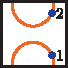
\includegraphics[scale=1]{CupCapDots.pdf}}}}}

\newcommand{\SigmaDotDot}{\mathord{\vcenter{\hbox{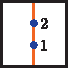
\includegraphics[scale=1]{SigmaDotDot.pdf}}}}}
\newcommand{\SigmaDotDotExchange}{\mathord{\vcenter{\hbox{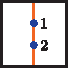
\includegraphics[scale=1]{SigmaDotDotExchange.pdf}}}}}
\newcommand{\TwoLine}{\mathord{\vcenter{\hbox{
\includegraphics[scale=1]{TwoLine.pdf}}}}}
\newcommand{\TwoLineDots}{\mathord{\vcenter{\hbox{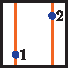
\includegraphics[scale=1]{TwoLineDots.pdf}}}}}

\newcommand{\RDotTwo}{\mathord{\vcenter{\hbox{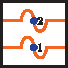
\includegraphics[scale=1]{RDotTwo.pdf}}}}}
\newcommand{\RDotTwoa}{\mathord{\vcenter{\hbox{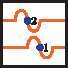
\includegraphics[scale=1]{RDotTwoa.pdf}}}}}
\newcommand{\RDotTwob}{\mathord{\vcenter{\hbox{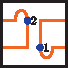
\includegraphics[scale=1]{RDotTwob.pdf}}}}}
\newcommand{\RDotTwoc}{\mathord{\vcenter{\hbox{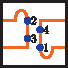
\includegraphics[scale=1]{RDotTwoc.pdf}}}}}

\newcommand{\FubeXXX}{\mathord{\vcenter{\hbox{
\includegraphics[scale=1]{EmptyTube.pdf}}}}}
\newcommand{\FubeXss}{\mathord{\vcenter{\hbox{
\includegraphics[scale=1]{OneLine.pdf}}}}}
\newcommand{\FubeXsds}{\mathord{\vcenter{\hbox{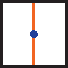
\includegraphics[scale=1]{OneLineDot.pdf}}}}}

\newcommand{\FubesXs}{\mathord{\vcenter{\hbox{
\includegraphics[scale=1,angle=90,origin=c]{OneLine.pdf}}}}}
\newcommand{\FubesdXs}{\mathord{\vcenter{\hbox{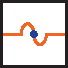
\includegraphics[scale=1]{FubesdXs.pdf}}}}}

\newcommand{\FubessX}{\mathord{\vcenter{\hbox{
\includegraphics[scale=1]{FubessX.pdf}}}}}
\newcommand{\FubessdX}{\mathord{\vcenter{\hbox{
\includegraphics[scale=1]{FubessdX.pdf}}}}}

\newcommand{\FubesXsa}{\mathord{\vcenter{\hbox{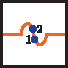
\includegraphics[scale=1]{FubesXsa.pdf}}}}}
\newcommand{\FubesXsb}{\mathord{\vcenter{\hbox{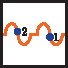
\includegraphics[scale=1]{FubesXsb.pdf}}}}}
\newcommand{\FubesXsc}{\mathord{\vcenter{\hbox{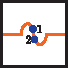
\includegraphics[scale=1]{FubesXsc.pdf}}}}}


\newcommand{\qqo}{\mathord{\vcenter{\hbox{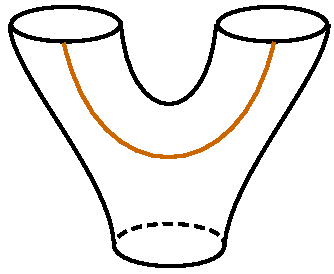
\includegraphics[scale=.4]{qq1.pdf}}}}}
\newcommand{\qtqo}{\mathord{\vcenter{\hbox{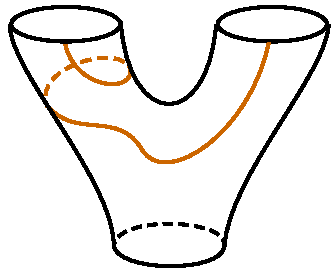
\includegraphics[scale=.4]{qtq1.pdf}}}}}
\newcommand{\qqto}{\mathord{\vcenter{\hbox{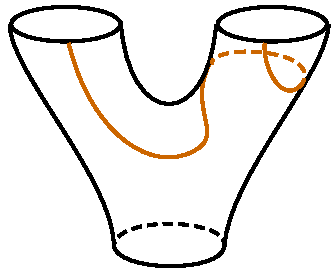
\includegraphics[scale=.4]{qqt1.pdf}}}}}
\newcommand{\qtqto}{\mathord{\vcenter{\hbox{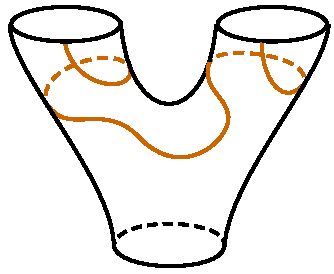
\includegraphics[scale=.4]{qtqt1.pdf}}}}}
\newcommand{\qqm}{\mathord{\vcenter{\hbox{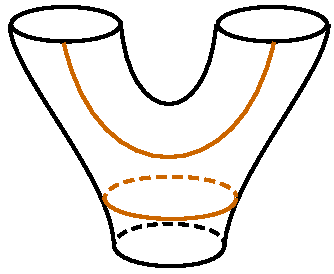
\includegraphics[scale=.4]{qqm.pdf}}}}}
\newcommand{\qtqm}{\mathord{\vcenter{\hbox{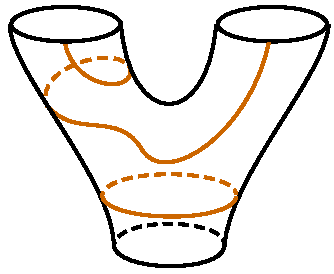
\includegraphics[scale=.4]{qtqm.pdf}}}}}
\newcommand{\qqtm}{\mathord{\vcenter{\hbox{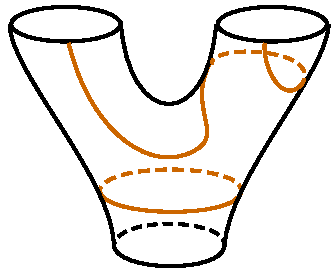
\includegraphics[scale=.4]{qqtm.pdf}}}}}
\newcommand{\qtqtm}{\mathord{\vcenter{\hbox{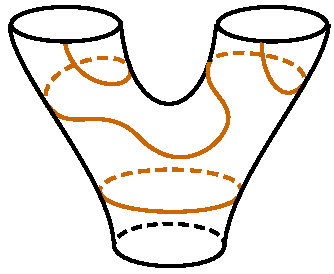
\includegraphics[scale=.4]{qtqtm.pdf}}}}}

\newcommand{\PantsPAP}{\mathord{\vcenter{\hbox{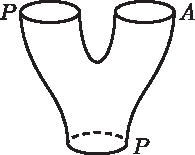
\includegraphics[scale=0.7]{PantsPAP.pdf}}}}}
\newcommand{\PantsPAsP}{\mathord{\vcenter{\hbox{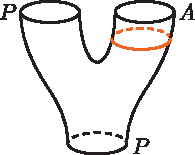
\includegraphics[scale=0.7]{PantsPAsP.pdf}}}}}

\newcommand{\PantsPsdAP}{\mathord{\vcenter{\hbox{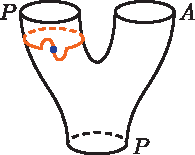
\includegraphics[scale=0.7]{PantsPsdAP.pdf}}}}}
\newcommand{\PantsPsdAsP}{\mathord{\vcenter{\hbox{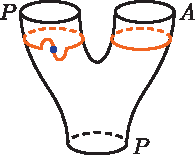
\includegraphics[scale=0.7]{PantsPsdAsP.pdf}}}}}



\newcommand{\PantsPPA}{\mathord{\vcenter{\hbox{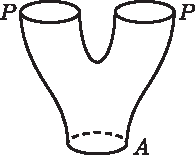
\includegraphics[scale=0.7]{PantsPPA.pdf}}}}}
\newcommand{\PantsPPAs}{\mathord{\vcenter{\hbox{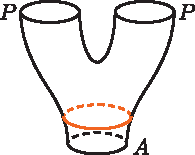
\includegraphics[scale=0.7]{PantsPPAs.pdf}}}}}

\newcommand{\PantsAsAshAsvt}{\mathord{\vcenter{\hbox{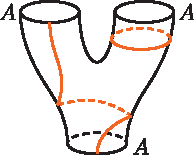
\includegraphics[scale=0.7]{PantsAsAshAsvt.pdf}}}}}
\newcommand{\PantsAstAAs}{\mathord{\vcenter{\hbox{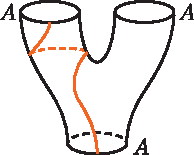
\includegraphics[scale=0.7]{PantsAstAAs.pdf}}}}}

\newcommand{\PantsAstAshAs}{\mathord{\vcenter{\hbox{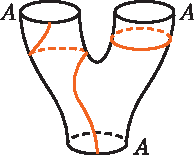
\includegraphics[scale=0.7]{PantsAstAshAs.pdf}}}}}
\newcommand{\PantsAsAshAs}{\mathord{\vcenter{\hbox{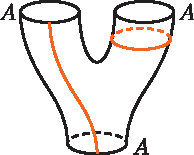
\includegraphics[scale=0.7]{PantsAsAshAs.pdf}}}}}
\newcommand{\PantsAsAAs}{\mathord{\vcenter{\hbox{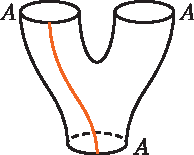
\includegraphics[scale=0.7]{PantsAsAAs.pdf}}}}}

\newcommand{\Pantssvtsvtsh}{\mathord{\vcenter{\hbox{
\includegraphics[scale=.7,origin=c]{Pantssvtsvtsh.pdf}}}}}
\newcommand{\Pantssvtsvsh}{\mathord{\vcenter{\hbox{
\includegraphics[scale=.7,angle=0,origin=c]{Pantssvtsvsh.pdf}}}}}
\newcommand{\Pantssvsvtsh}{\mathord{\vcenter{\hbox{
\includegraphics[scale=.7,angle=0,origin=c]{Pantssvsvtsh.pdf}}}}}
\newcommand{\Pantssvsvsh}{\mathord{\vcenter{\hbox{
\includegraphics[scale=.7,angle=0,origin=c]{Pantssvsvsh.pdf}}}}}
\newcommand{\PantssvtsvtX}{\mathord{\vcenter{\hbox{
\includegraphics[scale=.7,angle=0,origin=c]{PantssvtsvtX.pdf}}}}}
\newcommand{\PantssvtsvX}{\mathord{\vcenter{\hbox{
\includegraphics[scale=.7,angle=0,origin=c]{PantssvtsvX.pdf}}}}}
%\newcommand{\PantssvtsvX}{\mathord{\vcenter{\hbox{
\includegraphics[scale=.7,angle=0,origin=c]{PantssvtsvX.pdf}}}}}
\newcommand{\PantssvsvtX}{\mathord{\vcenter{\hbox{\includegraphics[scale=.7,angle=0,origin=c]{PantssvsvtX.pdf}}}}}
\newcommand{\PantssvsvX}{\mathord{\vcenter{\hbox{\includegraphics[scale=.7,angle=0,origin=c]{PantssvsvX.pdf}}}}}

\newcommand{\PantssvtXsvd}{\mathord{\vcenter{\hbox{\includegraphics[scale=.7,angle=0,origin=c]{PantssvtXsvd.pdf}}}}}
\newcommand{\Pantssvtshsvd}{\mathord{\vcenter{\hbox{\includegraphics[scale=.7,angle=0,origin=c]{Pantssvtshsvd.pdf}}}}}
\newcommand{\Pantssvshsvd}{\mathord{\vcenter{\hbox{\includegraphics[scale=.7,angle=0,origin=c]{Pantssvshsvd.pdf}}}}}
\newcommand{\PantssvXsvd}{\mathord{\vcenter{\hbox{\includegraphics[scale=.7,angle=0,origin=c]{PantssvXsvd.pdf}}}}}

\newcommand{\PantssvtXsvt}{\mathord{\vcenter{\hbox{\includegraphics[scale=.7,angle=0,origin=c]{PantssvtXsvt.pdf}}}}}
\newcommand{\PantssvXsvt}{\mathord{\vcenter{\hbox{\includegraphics[scale=.7,angle=0,origin=c]{PantssvXsvt.pdf}}}}}

\newcommand{\PantssvtXsv}{\mathord{\vcenter{\hbox{\includegraphics[scale=.7,angle=0,origin=c]{PantssvtXsv.pdf}}}}}

\newcommand{\PantssvXsv}{\mathord{\vcenter{\hbox{\includegraphics[scale=1,angle=0,origin=c]{PantssvXsv.pdf}}}}}

\newcommand{\TwoLinedotdot}{\mathord{\vcenter{\hbox{\includegraphics[scale=1.5,angle=0,origin=c]{TwoLinedotdot.pdf}}}}}

\newcommand{\Id}{\mathord{\vcenter{\hbox{\includegraphics[scale=1.5,angle=0,origin=c]{Id.pdf}}}}}

\newcommand{\CupSigmadot}{\mathord{\vcenter{\hbox{\includegraphics[scale=1.5,angle=0,origin=c]{Cupdot.pdf}}}}}

\newcommand{\CupSigma}{\mathord{\vcenter{\hbox{\includegraphics[scale=1.5,angle=0,origin=c]{Cup.pdf}}}}}

\newcommand{\StaggaredGSOdd}{\mathord{\vcenter{\hbox{\includegraphics[scale=1.5,angle=0,origin=c]{StaggaredGSOdd.pdf}}}}}
\newcommand{\StaggaredGSEven}{\mathord{\vcenter{\hbox{\includegraphics[scale=1.5,angle=0,origin=c]{StaggeredGSEven.pdf}}}}}

\newcommand{\StaggaredGSEvenR}{\mathord{\vcenter{\hbox{\reflectbox{\includegraphics[scale=1.5,angle=0,origin=c]{StaggeredGSEven.pdf}}}}}}





\newcommand{\VxsdsY}{\mathord{\vcenter{\hbox{\includegraphics[scale=0.3,angle=0,origin=c]{Vxsds.pdf}}}}}
\newcommand{\VsdxsY}{\mathord{\vcenter{\hbox{\includegraphics[scale=0.3,angle=0,origin=c]{Vsdxs.pdf}}}}}
\newcommand{\VtssdxY}{\mathord{\vcenter{\hbox{\includegraphics[scale=0.3,angle=0,origin=c]{Vtssdx.pdf}}}}}

\newcommand{\Vssdx}{\mathord{\vcenter{\hbox{\includegraphics[scale=0.3,angle=0,origin=c]{Vssdx.pdf}}}}}
\newcommand{\Vxsds}{\mathord{\vcenter{\hbox{\reflectbox{\includegraphics[scale=0.3,angle=0,origin=c]{Vssdx.pdf}}}}}}

\newcommand{\Vssx}{\mathord{\vcenter{\hbox{\includegraphics[scale=0.3,angle=0,origin=c]{Vssx.pdf}}}}}
\newcommand{\Vxss}{\mathord{\vcenter{\hbox{\reflectbox{\includegraphics[scale=0.3,angle=0,origin=c]{Vssx.pdf}}}}}}

\newcommand{\Vsxs}{\mathord{\vcenter{\hbox{\includegraphics[scale=0.3,angle=0,origin=c]{Vsxs.pdf}}}}}
\newcommand{\Vsxsd}{\mathord{\vcenter{\hbox{\includegraphics[scale=0.3,angle=0,origin=c]{Vsxsd.pdf}}}}}

\newcommand{\VsxsY}{\mathord{\vcenter{\hbox{\includegraphics[scale=0.3,angle=180,origin=c]{Vsxs.pdf}}}}}
\newcommand{\VssxY}{\mathord{\vcenter{\hbox{\includegraphics[scale=0.3,angle=180,origin=c]{Vssx.pdf}}}}}
\newcommand{\VxssY}{\mathord{\vcenter{\hbox{\reflectbox{\includegraphics[scale=0.3,angle=180,origin=c]{Vssx.pdf}}}}}}

\begin{document}


\title{Super lattice models dude}
\author{David Aasen, Ethan Lake, Kevin Walker, and Zhenghan Wang}
%\affiliation{Department of Physics and Astronomy, University of Utah, Salt Lake City, UT 84112, USA}
%\emailAdd{lake@physics.utah.edu}

\date{\today}

\maketitle

%\tableofcontents
\begin{abstract}
- fermion condensation/ Ising example

- modular transformations

- super-pivotal category

- exactly solvable Hamiltonian
\end{abstract}

\tableofcontents

\section{introduction}
- new phases of matter/other motivation

- fermion condensation as a method to generate super-pivotal categories

- explain how this differs from previous work. 

- emphasize tensoring over endo-morphisms

-  mention string nets from tubes picture/excitations

\section{Ising model}

- introduce Ising TQFT \cite{Lins1994}, and its graphical calculus with the $A$ factors

- condense fermions

- explain inconsistencies that necessitate spin structure, give physical interpretation of $p+ip$ SC.

- define spin structure and show why it's a phase of fermions. Mention that condensing $\psi$ couples the fermions and the Ising theory together 

- graphical calculus of condensed theory --- the constraint on $A^4$, how boxes work, moving dots around is $A^4$ from unitarity, etc

- give explicit example of why it's important to tensor over endomorphisms (e.g. getting endo space right)

- Drinfeld center of condensed theory: can briefly mention physical picture for why tubing (fubing?) works, talk about how this gets enlarged with spin stuff. Work through the identifications of each sector with the Clifford algebras 

- oddly isomorphic particles

- Fusion of quasi-particles --- include some (one or two?) examples of fusion spaces and how we do the calculation. 

- braiding of quasi-particles 

- modular transformations/relation to braiding data, filling in $S^3$, getting S matrix for all spin structures, philosophy about well-definedness of $S$ and $T$. 

- state sum???

The Ising TQFT, 


The idea is to notice that $1$ and $\psi$ form a fusion sub-algebra of the Ising fusion rules and so we can condense the $\psi$ particle by modding out this sub-algebra, provided that we introduce the spin structures needed to make this procedure legitimate. 

\begin{figure}
\includegraphics{folding_A3.pdf}
\caption{Performing the condensation from the Ising theory to the $C_2$ theory. The Dynkin diagram for $A_3$ folds about the node labeled by $\sigma$, producing the Dynkin diagram 
for $C_2$. The first node in the $C_2$ Dynkin diagram is the (fermionic) vacuum, and the second node is $\beta$, the image of $\sigma$ under condensation. } 
\end{figure}





In the case of the Ising model, any diagram with a $\psi$ line can be reduced to one where all the $\psi$ lines terminate on the defect. 
Thus in the target theory the only objects remaining will be $\sigma$ lines with possible fermions attached. We will write the image of $\sigma$ under the condensation procedure as $\Sigma$, and following Walker's notation, we will draw $\Sigma$ worldlines as 
\begin{align}
\FubeXss \qquad \qquad \FubeXsds,
\end{align}
where the dot denotes a $\psi$ ribbon which terminates on the sigma line and on the background spin-structure membrane. 

The process of removing two fermions results in a phase:
\begin{align}
\SigmaDotDot\; = A^4\; \FubeXss
\end{align}
where we take $A^4 = i$ (although $A^4 = -i$ is also fine). 
Exchanging fermions also results in a minus sign,
\begin{align}
\SigmaDotDot\;  &= - \; \SigmaDotDotExchange.
\end{align}
From the braiding endowed in the parent theory one ends up with some phases due to sliding the fermions past cups and caps in diagrams (should show this in more detail?)
\begin{align}
\CapDotRight\; &= - A^4 \; \CapDotLeft & \CupDotRight\; &=  A^4 \; \CupDotLeft.
\end{align}
These phases can be derived completely from the {\it braiding data} of the Ising theory, and must be such that going around a circular $\beta$ loop gives a factor of $-1$, which enforces the constraint that $A^8 = -1$. In more general examples, the braiding data in the parent theory will not be such that this is the case, this precludes an ability to have $q$-type objects with $\cl_1$ endomorphism algebras. 

The $F$-moves of the parent theory result in linear relations on the diagrams in the target theory
\begin{align}
\TwoLine\; & = \frac{1}{\sqrt{2}} \left( \CupCap \; + \;(A^4)^* \CupCapDots \right) \\
\CupCap \; &= \frac{1}{\sqrt{2}} \left(\TwoLine \; + \; \TwoLineDots \right).
\end{align}
%These are all the linear relations on the diagrams that we get.

The fubes are given by the string configurations 
\begin{align}
\FubeXXX \quad \FubesXs    \quad \FubeXss \quad \FubessX   \quad \FubesdXs \quad  \FubeXsds \quad \FubessdX
\end{align}
Each fube must come equipped with a spin structure, given by an element $\eta \in H^1(C,\zt) \cong \zt$, where $C$ is the cylinder. $\eta$ simply determines the nature of the boundary conditions for fermions which encricle the fube, and so the boundary conditions for fubes must obey a $\zt$ group structure. We have to be a little careful though, as mentioned earlier: contractible fermionic loops that twist fermion ribbons by $2\pi$ are associated with a $-1$ sign, and so the identity element in $H^1(C,\zt)$ corresponds to {\it anti-periodic} (or non-vorex) boundary conditions, with the nontrivial element corresponding to periodic (or vortex) boundary conditions.

We will denote the spin structure of a given fube with a subscript, either $A$ for anti-periodic/non-vortex sector or $P$ for periodic/vortex sector. 
Not every fube is consistent with each spin structure.
For example,
\begin{align}
\FubesdXs_A\;  = - \; \FubesdXs_A 
\end{align}
which follows from pulling the fermion around the boundary and so a minus sign is acquired. 
Meanwhile we have,
\begin{align}
\FubesXs_P \; = \; (A^4)^*\; \FubesXsa_P \; = (A^4)^* \; \FubesXsb_P =\;  (A^4)^* \FubesXsc_P \; = - \FubesXs_P.
\end{align}
All other fubes are nonzero for both spin structures.
Hence, a complete basis for fubes for the anti-peridioc sector is given by
\begin{align}
\FubeXXX_A \quad \FubesXs_A \quad \FubeXss_A \quad \FubessX_A    \quad  \FubeXsds_A \quad \FubessdX_A
\end{align}
while a basis for the periodic sector is given by,
\begin{align}
\FubeXXX_P\quad \FubeXss_P \quad \FubessX_P   \quad \FubesdXs_P \quad  \FubeXsds_P \quad \FubessdX_P
\end{align}

The tensor product in the fube algebra is given by stacking fubes and simplifying the resulting composite fube using local relations.  
For example, in the periodic sector we have
\begin{align}
\FubesdXs_P \; \times \; \FubesdXs_P \; = \; \RDotTwoa_P \; = \; \frac{1}{\sqrt{2}} \left(\RDotTwob_P + \RDotTwoc_P \right) = 2 \; \FubeXXX_P
\end{align}

Note that when we annihilate fermions into the vacuum to derive relations like this, we have to be careful about the order in which we do it, which is why we can never create two fermions side-by-side at the same time slice. For example, if we create fermion 1 above fermion 2 in a diagram, we must annihilate them along a $\Sigma$ string where fermion 1 is above fermion 2.
Also, note that since the spin structures on two fubes being fused must agree on the boundary at which they are being fused, periodic fubes only admit nonzero tensor products with periodic fubes, and similarly for anti-periodic fubes.

Relations like the ones above allow us to find the primitive central idempotents of the fube algebra, which carry the same information as the simple modules of the fube algebra, which in turn correspond to the vector spaces left invariant under the action of fube fusion\footnote{also known as {\it fubing}}, which we finally identify as quasiparticles. 

%The primitive central idempotents of an algebra $\mathcal{A}$ are given by a set $\Pi_a \in \mathcal{A}$ that satisfy: $\Pi_a \Pi_b = \delta_{ab} \Pi_a$ and $\Pi_a Q = Q \Pi_a$ for all $Q \in \mathcal{A}$, and each $\Pi_a$ cannot be decomposed as a sum of orthogonal idempotents. \ethan{Should we remove or relocate this paragraph?}

%\remove{Just realized we should probably have "odd" identity tubes, probbaly only in the periodic sector. They come from the tube in the parent theory which has a single fermion line. This in the target theory has $\psi$'s at the boundaries. We should then be able to cut it in half and the resulting tubes should still be elements of the tube algebra.}

\subsubsection{Kitaev wire}
\dave{This is actually really simple and super cool.}
\dave{Will need to find better notation for normal ordering and stuff.}
Here we propose a simple application of the above diagrammatic calculus. 
We will re-write the Kitaev-Majorana chain using this basis. 
The idea is to write down the natural anyon spin chain with this calculus and realize that it's exactly the Kitaev-Majorana chain. 
This elucidates the connection between Majorana zero modes and Ising anyons. 

The local ``on site" Hilbert space is spanned by two basis vectors
\begin{align}
    \CupSigma \qquad \text{and} \qquad \CupSigmadot
\end{align}
the first has even fermion parity, while the second has odd fermion parity.
The only terms one can contruct a Hamiltonian out of are
\begin{align}
\Id \qquad \text{and} \qquad \TwoLinedotdot
\end{align}
the first is the identity line, while the second is nontrivial and should be identified with $i \gamma_1 \gamma_2$, a Majorana bi-linear.
To see this, we can just check the action of the Hamiltonian on the basis vectors. 
\begin{align}
\TwoLinedotdot\; \times \; \CupSigma \; =\;  \CupSigma \quad \text{and} \quad \TwoLinedotdot\; \times \; \CupSigmadot \; =\;   - \; \CupSigmadot
\end{align}
\dave{Need to define ordering on vertices properly. I've been doing it by labeling the states first, then the operators have a natural ordering on them and I just begin counting from the last fermion on the state.}
For an $N$-site chain we have the basis of states,
\begin{align}
&\CupSigma \; \CupSigma \; \CupSigma \cdots \CupSigma\\
&\CupSigmadot \; \CupSigma \; \CupSigma \cdots \CupSigma\\
&\CupSigma \; \CupSigmadot \; \CupSigma \cdots \CupSigma\\
&\CupSigma \; \CupSigma \; \CupSigmadot \cdots \CupSigma\\
&\CupSigma \; \CupSigma \; \CupSigma \cdots \CupSigmadot\\
&\CupSigmadot \; \CupSigmadot \; \CupSigma \cdots \CupSigma
\end{align}
etcetera. Where there are $N$ cups appearing, and the fermion dots are ordered from right to left, and any number of them can appear.
If a state has an odd number of dots it has odd fermion parity, while an even number of dots has even fermion parity.
The Hamiltonian has two types of terms. One term mixes the states on site -- or within a single cup, while the other mixes nearest neighbour cups.
We will denote the onsite Hamiltonian terms by $H_{2j}$ and the the term which couples the nearest neighbour cups by $H_{2j+1}$.
Then the Hamiltonian takes on the form,
\begin{align}
H = - \sum_j\; t_j \; \;  \TwoLinedotdot_{\text{site $j$}}
\end{align}
Now in the completely staggered limit it's easy to see what the ground states are,
\begin{align}
\StaggaredGSEven \; \cdots \; \StaggaredGSEvenR  
\qquad \text{and} \qquad 
\StaggaredGSOdd \; \cdots  \; \StaggaredGSEvenR
\end{align}
The first differing from the second by fermion parity.
Excitations are built by putting dots on the intermediate cups. 
A nice feature of the diagrammatic notation is that the ``delocalization" of femrion number is made manifest.
For example the fermion odd state does not have a femrion localized at either end, rather its free to slide from one end to the other.
When transforming back to the original basis, one sees that the state is actually an even superposition of all possible placements of an even number of fermions, similarly for the odd state.
\dave{Sensible formula for JW transformation to get back to Ising?}

\subsection{Quasiparticle excitations}

To figure out the quasiparticle spectrum, we, as stated earlier, need to find the irreducible representations (or simple modules) of the tube algebra. Since the tube algebra splits into a direct sum of tubes with different spin structures, its simple modules will split in a similar way. First, we turn to an analysis of tubes with anti-periodic boundary counditions. 

\subsubsection{Anti-periodic sector}

Let us first examine the subalgebra of tubes with no charge: that is, cylinders with empty boundary conditions on both their top and bottom. Writing this subalgebra as $\tube_0^A$, we see that it is generated by two even tubes:
\be \tube_0^A = \left\langle\; \FubeXXX,\; \FubesXs\;\right\rangle.\ee
The odd tube with a horizontal $\beta$ line and a single fermion is zero, since taking the fermion once around the cylinder shows that it is equal to minus itself. 
Since $\tube_0^A$ has two even generators, as an algebra it must be isomorphic to $\cc^{2|0}$. The idempotents associated with this sector are easy to compute: $\cc^{2|0}$ has two simple modules and so we get two quasiparticles, which we label by $m_\unit$ and $m_\psi$. Explicitly, they are 
\be m_\unit = \frac{1}{2}\left( \FubeXXX_A +\;\; \frac{1}{\sqrt{2}}\FubesXs_A\right),\qquad m_\psi = \frac{1}{2} \left( \FubeXXX_A -\;\; \frac{1}{\sqrt{2}} \FubesXs_A\right).\ee
One can check that these idempotents are central, primitive, and orthogonal, and as such are associated with a pair of zero-charge quasiparticles. 

Now we turn to the subalgebra $\tube^A_\beta$ of charged tubes: those whose top and bottom boundary conditions consist of a single marked point. There are two non-zero even tubes and two non-zero odd tubes:
\be \tube^A_\beta = \left\langle\; \FubeXss,\;\FubeXsds,\; \FubessX,\; \FubessdX\right\rangle,\ee
meaning that as an algebra, $\tube^A_\beta \cong \cc^{2|2}$. $\cc^{2|2}$ is isomorphic to both $\cl_2$ and $\cl_1\oplus \cl_1$, and so we know that this sector will contribute either one (if $\cl_2$) or two (if $\cl_1^{\oplus 2}$) quasiparticle excitations. 

In order to identify the idempotents of this subalgebra, we need to write down the multiplication rules. By using the local relations in the $C_2$ theory we can work out the multiplication table as follows, where $A\tp B$ means ``stack $A$ on top of $B$'', and where we always take fermions in the $A$ tube to have a larger normal order than fermions in the $B$ tube:
\be
\renewcommand{\arraystretch}{3}
\begin{tabular}{c | c c c c r}
$\times$ in $\tube^A_{\beta} $          & $\FubeXss $ & $\FubeXsds $ & $\FubessX $&$ \FubessdX$  \\
\hline
$\FubeXss$ & $\FubeXss$ & $\ \FubeXsds$  & $\FubessX$ & $\FubessdX$  \\

$\FubeXsds$           & $\FubeXsds $& $i\ \FubeXss$ & $\FubessdX $& $i\ \FubessX  $\\

$\FubessX$          & $\FubessX $&$ -\ \FubessdX  $&$ e^{-i\pi/4}\ \FubeXss $&$ -e^{-i\pi/4}\ \FubeXsds $\\

$\FubessdX    $&$ \FubessdX $&$ -i\ \FubessX $&$ e^{-i\pi/4}\ \FubeXsds $&$ -e^{i\pi/4}\ \FubeXss$   \\
\end{tabular}
\ee
Note that in the above table, we've taken $A^4 = i$ for concreteness. Since the multiplication table is non-abelian, this algebra must be $\cl_2$, as $\cl_1\oplus\cl_1$ is abelian. 
In order to show that this is indeed the multiplication table of $\cl_2$, we perform the following re-scaling:
\be \FubeXsds \mapsto e^{-\pi i/4} \FubeXsds,
\qquad \FubessX \mapsto e^{5\pi i/8} \FubessX,\qquad \FubessdX \mapsto e^{3\pi i/8} \FubessdX.\ee
With this, the re-scaled multiplication table becomes 
\be
\renewcommand{\arraystretch}{3}
\begin{tabular}{c | c c c c r}
$\times$ in $\tube^A_{\beta} $          & $\FubeXss $ & $\FubeXsds $ & $\FubessX $&$ \FubessdX$  \\
\hline
$\FubeXss$ & $\FubeXss$ & $\FubeXsds$  & $\FubessX$ & $\FubessdX$  \\
$\FubeXsds$           & $\FubeXsds $& $\FubeXss$ & $\FubessdX $& $\FubessX  $\\
$\FubessX$          & $\FubessX $&$ -\FubessdX  $&$ -\FubeXss $&$ \FubeXsds $\\
$\FubessdX    $&$ \FubessdX $&$ -\FubessX $&$ -\FubeXsds $&$ \FubeXss$   \\
\end{tabular}
\ee
Recall that $\cl_2$ has two even generators $1$ and $\gamma_1\gamma_2$, and two anticommuting odd generators $\gamma_1$ and $\gamma_2$ that square to $1$. We see that if we make the identifications
\be 1 =\FubeXss,\quad \gamma_1 =  \FubeXsds,\quad \gamma_2 = \FubessdX,\quad i\gamma_1\gamma_2 =  \FubessX,\ee
we have the required anticommutation relations $\{\gamma_1,\gamma_2\} = 0$, as well as the identities $\gamma_1^2 = \gamma_2^2 = 1$, and so indeed, $\tube^A_\beta \cong \cl_2$. 
%Since we have $c^\dagger c = i\gamma_1\gamma_2$ if $c = (\gamma_1 + i\gamma_2)/\sqrt{2}$, we have the intriguing relation 
%\be c^\dagger c = \FubessX.\ee
%That is, we see that the number operator is equal to the tube that implements the twist. This actually makes sense: each fermion on an anti-periodic tube gives a factor of $-1$ when twisted, and so twisting tubes gives a way of computing the (physical) fermion parity of the tube. 

We now turn to the task of identifying the quasiparticles (simple modules) of this algebra. 
Because of the Morita equivalence between $\cl_2$ and $\cc$, $\cl_2$ and $\cc$ must have the same simple modules (idempotents), and so the subalgebra $\tube^A_\beta$ must correspond to only one type of quasiparticle.

To see this directly, we note that since $\cl_2 \cong \End(\cc^{1|1})$, its simple modules (quasiparticles) can each be identified with the space $\cc^{1|1}$. It's easy to check that there are two different simple modules which we write as $m^{\pm}$, corresponding to the representations of $\cl_2$ $\rho^\pm : \cl_2 \ra \Aut(\cc^{1|1})$ given by $\rho^\pm(1) = \sigma^0,\rho^\pm(\gamma_1) = \sigma^x,$ and $\rho^\pm(\gamma_2) = \pm i\sigma^y$, where the $\gamma_i$ maintain their earlier identifications. This means that the two quasiparticle types $m^\pm$ associated with the two representations differ in the sign of the representation matrix of $\gamma_2$, meaning that we can write them as
\be m_\sigma^\pm = \frac{1}{2} \left(\FubeXss_A \pm e^{i\pi/8}\ \FubessX_A\right),\ee
since the second tube in the above expression is oddly isomorphic to $\gamma_2$. Note that we're letting each fube in the above expression represent its isomorphism class, which is why we haven't added any fubes in $\fld(C)^1$ with odd fermion parity to the expression for $m_\sigma^\pm$ (as they are isomorphic to the even-parity fubes in the expression for $m^\pm$) . 

This looks to give us two quasiparticles, which is a contradiction. The resolution to this is that the two simple modules $m^\pm$ are actually {\it oddly isomorphic} to one another, by virtue of the anti-periodic spin structures they possess. Creating a fermion on the top of the $\gamma_2$ tube (which corresponds to the isomorphism given by left multiplication by $\gamma_1$), dragging it around the $\gamma_2$ tube to the bottom, and then annihilating it (through the isomorphism given by right multiplication by $\gamma_1$) acts on the matrix representations as  $\rho^\pm(\gamma_2) \mapsto \rho^\mp(\gamma_2)$, and thus establishes an isomorphism $m^+\cong m^-$. Since only isomorphism classes of quasiparticles are physical, we can therefore identify the two modules $m_\sigma^\pm$ with a single quasiparticle. In what follows, we will choose $m_\sigma^+$ as the representative for the isomorphism class. 

We will examine the fusion rules and braiding properties of the three quasiparticles identified so far later. For now, we repeat our quasiparticle identification procedure for quasiparticles in the vortex sector, which possess spin structures with periodic boundary conditions around the cylinder. 

\subsubsection{Periodic (vortex) sector}

$\cl_1$ has only one simple module, namely $\cc^{1|1}$ with the matrix representation $\rho(1) = \sigma^0,\rho(\gamma)=\sigma^x$, and so will support only one quasiparticle

The explicit presentation for the $\cl_1$ quasiparticle is a bit more subtle. Since $\fld^P(C)$ is a graded superspace, we are prevented from adding field configurations with different fermion parity, and thus cannot form superpositions of the tubes in $\fube^P_0$. However, we note that in $\cl_1$, $1$ and $\gamma$ are isomorphic through multiplication by $\gamma$, which establishes an (odd) isomorphism between the two basis vectors in $\fube^P_0$. Since only isomorphism classes of field configurations are physical, we can identify the two fubes with one another, which form an orbit under multiplication by $\gamma$. For definiteness we will choose to represent this isomorphism class by the even-parity sector, and so we write the $\cl_1$ quasiparticle as (really? or just say idempotents have to be even?)
\be q_\sigma = \FubeXXX_P.\ee








Now for the periodic spin structure, corresponding to the subalgebra $\fube_\Sigma^P$. The multiplication table for $\fube_\Sigma^P$ is the same as the one for the $\fube_\Sigma^A$, modulo a few minus signs and conjugations. Explicitly, we obtain
\be
\renewcommand{\arraystretch}{3}
\begin{tabular}{c | c c c c r}
$\tp$ in $\fube^P_{\Sigma} $          & $\FubeXss $ & $\FubeXsds $ & $\FubessX $&$ \FubessdX$  \\
\hline

$\FubeXss$ & $\FubeXss$ & $ \FubeXsds$  & $\FubessX$ & $\FubessdX$  \\

$\FubeXsds$           & $\FubeXsds $& $i\ \FubeXss$ & $\FubessdX $& $i\ \FubessX  $\\

$\FubessX$          & $\FubessX $&$ \ \FubessdX  $&$ e^{i\pi/4}\ \FubeXss $&$ e^{i\pi/4}\ \FubeXsds $\\

$\FubessdX    $&$ \FubessdX $&$ i\ \FubessX $&$ e^{i\pi/4}\ \FubeXsds $&$ e^{i3\pi/4}\ \FubeXss$   \\
\end{tabular}
\ee

As in the anti-periodic, we can do a re-scaling of the tubes to make the underlying algebraic structure more transparent. The most convenient re-scaling is 
\be \FubeXsds \mapsto e^{-\pi i/4} \FubeXsds,
\qquad \FubessX \mapsto e^{\pi i/8} \FubessX,\qquad \FubessdX \mapsto e^{-\pi i/8} \FubessdX.\ee
With this choice of re-scaling, the re-scaled multiplication table for $\fube_\Sigma^P$ is the same as re-scaled one for $\fube_\Sigma^A$, expect there are no minus signs, meaning that $\fube_\Sigma^P$ is commutative. Since we argued earlier that the only choices for $\fube_\Sigma^{A/P}$ were $\cl_1\oplus\cl_1$ or $\cl_2$, commutativity implies that we can set $\fube_\Sigma^P \cong \cl_1\oplus\cl_1$. To check this we need to do a little manipulation, since the multiplication table for $\fube_\Sigma^P$ doesn't look like a direct sum of two $\cl_1$ multiplication tables at first glance. To fix notation, we will write the two odd generators in $\cl_1\oplus\cl_1$ as $\gamma^+$ and $\gamma^-$, and the even generators as $1^+, 1^-$. If we define these generators in terms of the fubes by (keeping the phases explicit)
\be \unit^\pm = \frac{1}{2}\left(\FubeXss \pm e^{-i\pi/8}\FubessX\right),\qquad   \gamma^\pm = \frac{e^{-i\pi/4}}{2}\left(\FubeXsds \pm e^{-i\pi/8}\FubessdX\right)\ee
and then re-write the multiplication table for $\fube_\Sigma^P$, we see that we indeed get a $\langle \unit^+ ,\gamma^+\rangle \oplus \langle \unit^- \oplus \gamma^-\rangle =\cl_1\oplus\cl_1$ structure with $(\gamma^\pm)^2 = \unit^\pm$. Thus, there are two $\cl_1$-type quasiparticles corresponding to the $\fube_\Sigma^P$ subalgebra. Again, since only isomorphism classes of fubes are physical, we can write the two $\cl_1$-type quasiparticles in terms of even-parity fubes only:
\be q_\unit = \unit^+,\qquad q_\psi = \unit^-.\ee

\subsection{Obtaining the quasiparticle fusion rules}

With all idempotents at hand we are in a place to compute the fusion rules. The process is the same as discussed in Section \ref{FindingFusionRules}.
We take three idempotents and ask if there exists a linear combination of pants that will take two of the idempotents to the third. The number of linearly independant maps gives the fusion multiplicity.
Computationally it is easier to search for pairs of pants that are invariant under application of each idempotent. 
For example, suppose we wanted to find the fusion rule for $q_\sigma \otimes m_1$.
We first note that the spin structure boundary conditions require that they fuse to a vortex (a fube with a periodic spin structure). Furthurmore, since both $m_1$ and $q_\sigma$ have flux and no charge, we know that the pants cannot have any charge lines. Since there is only one resulting fube that has no charge lines and periodic  boundary conditions, namely $q_\sigma$, we know that the pair of pants desribing the fusion $q_\sigma \otimes m_1$ is the supervector space with even generator
\begin{align}
\fld_{q_\sigma\tp m_1}^{q_\sigma}(Y; \text{even}) = \left\langle \PantsPAP \; +\;  \frac{1}{\sqrt{2}} \PantsPAsP \right \rangle
\end{align}
and odd generator
\begin{align}
\fld_{q_\sigma\tp m_1}^{q_\sigma}(Y;  \text{odd}) = \left\langle \PantsPsdAP \; +\;  \frac{1}{\sqrt{2}} \PantsPsdAsP \right \rangle
\end{align}
\dave{add note about moving dot from top leg to bottom.}
and the fusion rule is $q_\sigma \otimes m_1 = q_\sigma$.
Similarly the supervector space $\fld_{q_\sigma \tp m_\psi}(Y)$ has one even generator
\begin{align}
\fld_{q_\sigma\tp m_\psi}(Y) = \left\langle \PantsPAP \; - \; \frac{1}{\sqrt{2}} \PantsPAsP \right \rangle
\end{align}
and the analgous odd generator
and therefore $q_\sigma \tp m_\psi = q_\sigma$.
\dave{Fix to include odd generators as well in rest of section.}
A more nontrivial example is to consider the tensor product of two $q_\sigma$ idempotents.
This again has no charge, but the resulting tube can have either flux, 
\begin{align}
\fld_{q_\sigma\tp q_\sigma}(Y) &= \left\langle \PantsPPA \; +\;  \PantsPPAs \right \rangle\\
&= \left\langle \PantsPPA  + \frac{1}{\sqrt{2}} \PantsPPAs \right \rangle \bigoplus \left\langle \PantsPPA  - \frac{1}{\sqrt{2}} \PantsPPAs \right \rangle
\end{align}
where in the second line we have decomposed the first line into pants that are invariant under application of $m_1$ and $m_\psi$. 
This demonstrates the fusion rule $q_\sigma \tp q_\sigma = m_1 \oplus m_\psi$. 
Slightly more non-trivial fusion rules follows from $m_\sigma^{\pm} \tp m_\psi$ and $m_\sigma^{\pm} \tp m_\psi$. 
The idempotent $m_\psi$ is purely flux, and so the pants can only have pure flux degrees of freedom on the leg matching the $m_\psi$ idempotent. $m_\sigma^{\pm}$ also has charge. 
Hence the idempotent resulting from from fusion will also have charge and again have anti periodic boundary conditions.
One finds that the $m_\sigma$ idempotent can be slipped up the pair of pants with the expense of introducing a $\sigma$ line around the other leg,
\begin{align}
\PantsAstAAs  = \frac{1}{\sqrt{2}} \;  \PantsAsAshAsvt
\end{align}
Now one can check that $m_\psi$ is an eigenstate of the closed sigma loop with eigenvalue $-\sqrt{2}$ and $m_1$ is an eigenstate with eigenvalue $+\sqrt{2}$. Hence one finds that $m_\sigma^{\pm} \tp m_\psi  = m_\sigma^{\mp} \cong m_\sigma^\pm$ and $m_\sigma^{\pm} \tp m_1 = m_\sigma^{\pm}$. 
Hence we can write, for example,
\begin{align}
\fld_{m_\sigma^{\pm} \tp m_\psi}^{m_\sigma^{\mp}}(Y) = \left\langle \PantsAsAAs -\frac{1}{\sqrt{2}}\PantsAsAshAs \pm \PantsAstAAs  \mp \frac{1}{\sqrt{2}} \PantsAstAshAs   \right \rangle
\end{align}
Since the $m_\sigma^{+}$ is isomorphic to to $m_\sigma^-$ we can always choose to work with either $m_\sigma^+$ or $m_\sigma^-$. In this case we can write,
\begin{align}
\fld_{m_\sigma^{+} \tp m_\psi}^{m_\sigma^{+}}({}^AY_A^A, \text{odd}) = \left\langle \PantssvXsvd -\frac{1}{\sqrt{2}}\Pantssvtshsvd + \PantssvtXsvd  - \frac{1}{\sqrt{2}} \Pantssvshsvd   \right \rangle 
\end{align}

The trickiest is $m_\sigma^\pm \tp m_{\sigma}^\pm$. For these we have, 
\begin{align}
\text{\dave{some pants}} &=      \Pantssvtsvtsh
\Pantssvtsvsh
\Pantssvsvtsh
\Pantssvsvsh \\
&\PantssvtsvtX
\PantssvtsvX
\PantssvsvtX
\PantssvsvX
\end{align}
\begin{align}
    \fld_{m_\sigma^{+} \tp m_\sigma^+}^{m_1}({}^AY_A^A; \text{even} ) &= \left \langle \PantssvsvX +  \frac{1}{\sqrt{2}}\Pantssvsvsh +\PantssvsvtX +\frac{1}{\sqrt{2}} \Pantssvsvtsh \right \rangle
\end{align}
\begin{align}
    \fld_{m_\sigma^{+} \tp m_\sigma^+}^{m_\psi}({}^AY_A^A; \text{even} ) &= \left \langle \PantssvsvX -  \frac{1}{\sqrt{2}}\Pantssvsvsh +\PantssvsvtX -\frac{1}{\sqrt{2}} \Pantssvsvtsh \right \rangle
\end{align}
and the odd ones are given by putting a single dot on the upper left leg.

\dave{More pants}
\begin{align}
\fld_{q_1 \tp m_\sigma^+}^{q_\sigma}({}^PY_P^A; \text{even} ) = \left \langle 
\PantssvsvX + 
\PantssvtsvX+
\PantssvsvtX+
\PantssvtsvtX \right \rangle
\end{align}
\dave{The odd pants come from adding a dot to top left leg. These should be verified.}
\begin{align}
\fld_{m_\sigma^+ \tp q_\sigma}^{q_1}({}^PY_P^A; \text{even} ) = \left \langle
\PantssvtXsvt+
\PantssvXsvt+
\PantssvtXsv+
\PantssvXsv \right \rangle
\end{align}
\begin{align}
\fld_{m_\sigma^+ \tp q_\sigma}^{q_1}({}^PY_P^A; \text{even} ) = \left \langle
\PantssvXsv+
\PantssvtXsv+
\PantssvXsvt+
\PantssvtXsvt \right \rangle
\end{align}
\begin{align}
\fld_{m_\sigma^+ \tp q_\sigma}^{q_\psi}({}^PY_P^A; \text{even} ) = \left \langle
\PantssvXsv+
\PantssvtXsv-
\PantssvXsvt-
\PantssvtXsvt \right \rangle
\end{align}

We summarize the fusion rules in the following table: 
\begin{table}
\resizebox{\linewidth}{!}{%
\begin{tabular}{c||c|c|c||c|c|c}
$ {A\otimes B} $&$m_\unit $&$m_\sigma^+$&$m_\psi$&$q_\unit$&$q_\sigma$&$q_\psi $\\
     \hline
     \hline
     
$m_\unit $&$m_\unit$&$ m_\sigma^+$&$m_\psi$&    $\bullet q_\unit$&$\bullet q_\sigma$&$\bullet q_\psi$ \\

     \hline
$m_\sigma^+ $&$m_\sigma^+$&$\cc^{1|0}m_\unit \oplus \cc^{0|1}m_\psi $&$ m_\sigma^+ $&$      \bullet q_\sigma $&$ \bullet q_\unit$&$ \bullet q_\sigma$ \\

% $$&$$&$$&$$&$$&$q_\psi$&$$\\
     \hline
     
$m_\psi $&$m_\psi$&$m_\sigma^+$&$m_\unit$&      $\bullet q_\psi$&$\bullet q_\sigma$&$\bullet q_\unit $\\

     \hline
     \hline
     
$q_\unit $&$\bullet q_\unit$&$\bullet q_\sigma $&$\bullet q_\psi$&$\bullet m_\unit$&$\bullet m_\sigma^+$&$\bullet m_\psi$\\

\hline
$q_\sigma$&$\bullet q_\sigma$&$\bullet (q_\unit \oplus q_\psi)$&$\bullet q_\sigma$&$\bullet m_\sigma^+$&$\bullet (m_\unit \oplus m_\psi)$&$\bullet m_\sigma^+$ \\

%$                $&$$&$q_\psi$&$$&$$&$m_\psi$&$$ \\

\hline
$q_\psi $&$\bullet q_\psi$&$\bullet q_\sigma$&$\bullet q_\unit$&$\bullet m_\psi$&$\bullet m_\sigma^+$&$\bullet m_\unit$
\end{tabular}
}
\caption{The quasiparticle fusion rules in $\mcz(C_2)$. Bullets in front of indicate that the associated fusion space is isomorphic to $\cc^{1|1}$. The $m_\sigma^+ \tp m_\sigma^+$ entry indicates that the fusion space can either be even if the fusion product is $m_1$, or purely odd (isomorphic to $\cc^{0|1}$) if the fusion product is $m_\psi$. }
\end{table}


\section{Braiding data}

 
\subsection{$R$-matrices}
In this subsection we provide a table of the $R$ symbols in the theory. First, we need to set some conventions on our fusion spaces. We will work on the three-punctured sphere rather than drawing out pairs of pants, as it is much easier to perform calculations using the three-punctured sphere picture. 

We will write a generic even fusion space, which is an even vector in the fusion space $\fld^{a,b}_c$, as 
\be \label{pants_braiding_basis} \includegraphics{pants_braiding_basis.pdf},\ee
where $a,b,c\in \mcz(C_2)$ and $u,v,w\in \zt$ are variables indicating whether or not a $\beta$ line is present on the given link. The idempotent labels represent a collection of pictures, one for each tube in their definition. For example, 
\be \includegraphics{msig_def.pdf} \ee

We will calculate the braiding in the fusion space $\fld^{a,b}_c$ by moving the $a$ and $b$ punctures around one other and re-expressing the result in terms of the basis vectors in $\fld^{b,a}_c$. When braiding $q$-type particles, we enforce their periodic boundary conditions graphically by introducing branch cuts ending on each $q$-type puncture, with the rule that dots sliding past a branch cut pick up a phase of $-1$. For concreteness, we will draw our branch cuts to always meet near the center of the three punctures. For example, to calculate $R^{q_\psi q_{1/\psi}}_{m_{\psi/1}}$, we write
\be \includegraphics{qpsiq1psi_braiding} \ee
where the dashed blue lines are the branch cuts, and we have taken advantage of our knowledge of the eigenvalue of $q_\psi$ under the twisted tube (i.e. the spin of $q_\psi$). 

We define odd vectors in $\fld^{a,b}_c$ by placing dots on the top left leg of the pants, on the leg marked $u$ in \eqref{pants_braiding_basis}. If this is impossible (e.g. if the top left leg is an $m_\psi$ idempotent), we put the dot on the top right leg of the pants, marked $v$ in \eqref{pants_braiding_basis}. For example, we can calculate the $R$-symbol $R^{m_\psi m_\sigma^+}_{m_\sigma^+} = -1$ by
\be \includegraphics{mpsimsig_braiding.pdf}.\ee
A slightly more complicated example is the odd fusion channel in $R^{q_\psi q_{1/\psi}}_{m_{\psi/1}}$:
\be \includegraphics{qpsiq1psidot_braiding.pdf} \ee
Note that we have assumed we can ``pivot'' branch cuts around the punctures on which they are located, provided that we pick up a factor of $-1$ each time the branch cut crosses a fermion. 

We have to remember to always move the dots back to the left side of the pants after the braid takes place, if possible. As an example, we can calculate the braiding of the odd fusion channel in $R^{q_\sigma q_{1/\psi}}_{m_\sigma^+}$:
\be \includegraphics{qsigq1psidot_braiding.pdf} \ee


Hopefully these examples convey the general idea of how to work out the full table of $R$-symbols, which we present below. 
The tables of values below denotes the row braiding entry over the top of the column entry, and so is of the form
\begin{tabular}{c|c}
     & B\\
     \hline
A     & $R^{AB}_{A\otimes B}$
\end{tabular}
Dots in the table indicate odd fusion channels. 

\resizebox{\linewidth}{!}{%
\begin{tabular}{c||c|c|c||c|c|c}
$     R^{AB}_{A\otimes B} $&$m_\unit $&$m_\sigma^+$&$m_\psi$&$q_\unit$&$q_\sigma$&$q_\psi $\\
     \hline
     \hline
     
$m_\unit $&$m_\unit$&$ m_\sigma^+$&$m_\psi$&    $(1+1\bullet)q_\unit$&$(1+1\bullet)q_\sigma$&$(1+1\bullet)q_\psi$ \\ %yup

     \hline
$m_\sigma^+ $&$m_\sigma^+$&$\zeta^{-1}(m_\unit-i\bullet m_\psi) $&$ \bullet m_\sigma^+ $&$      \zeta^{-1}(1+i \bullet)q_\sigma $&$ (1-\zeta^2/d\bullet ) q_\unit$&$ \zeta^{-1}(1+i\bullet)q_\sigma$ \\

 $$&$$&$$&$$&$$&$+(1+\zeta^2/d\bullet) q_\psi$&$$\\
     \hline
     
$m_\psi $&$m_\psi$&$(-1\bullet) m_\sigma^+$&$m_\unit$&      $-(1+ 1\bullet)q_\psi$&$(1+1\bullet )q_\sigma$&$-(1+1\bullet)q_\unit $\\

     \hline
     \hline
     
$q_\unit $&$(1+1\bullet)q_\unit$&$\zeta(1-i \bullet)q_\sigma $&$(1+1\bullet)q_\psi$&$\zeta(1+i \bullet)m_\unit$&$(1+ \zeta^{-2}/d \bullet )m_\sigma^+$&$\zeta(1+i \bullet)m_\psi$\\

\hline
$q_\sigma $&$(1+1\bullet)q_\sigma$&$(\zeta^{-2}- d i \bullet)q_\unit$&$(1+1\bullet)q_\sigma$&$(\zeta^2+i d \bullet )m_\sigma^+$&$(1+i\bullet) m_\unit$&$(-\zeta^2+i d \bullet)m_\sigma^+$ \\

$                $&$$&$(-\zeta^{-2}- d i \bullet)q_\psi$&$$&$$&$+(1-i\bullet)m_\psi$&$$ \\

\hline
$q_\psi $&$(1+1\bullet)q_\psi$&$-\zeta(1-i\bullet)q_\sigma$&$(1+1 \bullet)q_\unit$&$-\zeta(1+i\bullet)m_\psi$&$(1-\zeta^{-2}/d \bullet )m_\sigma^+$&$-\zeta(1+i \bullet)m_\unit$
\end{tabular}
}
\\ \ \\
For convenience, we have defined 
\be \zeta := e^{-i\pi/8} = \theta_{m_\sigma^+}.\ee
If we switched the choice for $A^4$ (e.g. from $i$ to $-i$), we could obtain the switched $R$-symbols by sending $\zeta \mapsto \zeta^*$. 

\subsection{Twists}

There are three ways to compute the twist: by statistics (braiding two identical idempotents around one another), by spin (applying Dehn twists on the idempotents), and by modular transformations (by performing Dehn twists on the torus). 

We'll start by computing the twists by statistics, namely by tracing out the $R$ symbols. 
First for the $m$ sector. 
If we use the normal trace, we obtain 
\be \theta_{m_\unit} = 1,\ \theta_{m_\psi} = 1,\ \theta_{m^\pm_\sigma} = \pm e^{-i\pi/8}.\ee
If we use the supertrace instead, we get 
\be \theta_{m_\unit} = 1,\ \theta_{m_\psi} = 1,\ \theta_{m^\pm_\sigma} = \pm e^{3i\pi/8}.\ee
Now for the $q$ sector. If we use the trace, we get 
\be \theta_{q_\unit} = e^{i\pi/8},\ \theta_{q_\psi} = -e^{i\pi/8},\ \theta_{q_\sigma} = 1,\ee
while if we use the supertrace, we get 
\be \theta_{q_\unit} = e^{-3i\pi/8},\ \theta_{q_\psi} = -e^{-3i\pi/8},\ \theta_{q_\sigma} = 1.\ee

Now we will compute the spins of the idempotents by Dehn-twisting each of their tubes. This can be done by looking at the tube algebra multiplication tables for each of the periodic and anti-periodic sectors. 
For the anti-periodic sector, we obtain 
\be \theta_{m_\unit} = 1,\ \theta_{m_\psi} = 1,\ \theta_{m^\pm_\sigma} = \pm e^{-i\pi/8}.\ee
For the periodic (vortex) sector, we obtain 
\be \theta_{q_\unit} = e^{i\pi/8},\ \theta_{q_\psi} = -e^{i\pi/8},\ \theta_{q_\sigma} = 1.\ee
Note that the $T$-matrix in the vortex sector decomposes as 
\be T_P = T_{p+ip} \tp T_{\text{Ising}^{\nu = -1}},\ee
agreeing with previous results which computed the modular transformations on the periodic-periodic torus, and hinted at the existence of a secret $p+ip$ superconductor in the vortex sector. Additionally, notice that if we want to have spin-statistics hold, we need to {\it trace} out the $R$-symbols, not supertrace them.

In the expressions above, the twists of every non-vortex $m$-type particle are ambiguous up to a factor of $\pm1$, corresponding to an ambiguity in the parity of physical fermions (boxes) attached to the tubes at the time of twisting. In this picture, the $q$-type particles have no such ambiguity, since moving an extra physical fermion around a periodic tube incurs no $-1$ sign as a result.  
If we believe that the philosophy behind the expression for chiral central charge familiar from the bosonic case goes through unchanged in the superfusion case, we should have $c_-=0$ for this theory, since we can realize this phase in a lattice model. This is sort of trivially true for the non-vortex sector, since the twists being only defined up to $\pm1$ mean that the sum over twists ``averages out'' and becomes zero. The constraint on $c_-=0$ is a nontrivial constraint for the vortex sector though, since the twists there are fully determined. Of course, by looking at the list of twists, we see that the vortex sector is indeed non-chiral. Physically, there are hints that the $c_-=-1/2$ of the Ising theory (which would be $c_- = 1/2$ if we chose $A^4=-i$) is cancelled by the $c_-=1/2$ of a background $p+ip$ superconductor that came along with the fermions we added to equip the theory with a spin structure. 

\subsection{Topological $S$-matrix}
\subsubsection{From braiding}

Having obtained the $R$ symbols, we can now go ahead and calculate the $S$-matrix. To do this, we will use the following quantum dimensions: 
\be d_{m_1} = d_{m_\psi} = 1,\quad d_{m_\sigma^+} = d_{q_1} = d_{q_\psi} = \sqrt{2},\quad d_{q_\sigma} = 2,\ee
which gives $\mcd = \sqrt{12}$.

There are several ways to calculate $S$. For all of them, we should keep in mind that although there are some $\pm1$ ambiguities in $T$, such ambiguities should not be present in $S$, since fermions have trivial double-braiding with one another. That is, mapping $m_a \mapsto fm_a$ where $a\in \{\unit,\psi,\sigma\}$ and $f$ is a physical fermion should not affect the answer we get for the $S$-matrix. In what follows we will calculate the $S$-matrix in several different ways, and then use a handful of different arguments to figure out what each calculation means. 

First, we can calculate $S$ by tracing out the $R$-symbols, using 
\be S_{ab} = \frac{1}{\mcd}\sum_{c}d_c{\rm Tr}[R^{ab}_cR^{ba}_c],\ee
where ${\rm Tr}$ is the trace, not the supertrace. This gives 
\be 
 S^{Tr} = \frac{1}{\mcd} \begin{pmatrix} 
1&\sqrt{2}&1&2\sqrt{2}&4&2\sqrt{2} \\
 \sqrt{2}&0&-\sqrt{2}&4&0&-4 \\ 
 1&-\sqrt{2}&1&-2\sqrt{2}&4&-2\sqrt{2} \\ 
 2\sqrt{2}&4& -2\sqrt{2}&0&0&0 \\ 
 4&0&4&0&0&0 \\ 
  2\sqrt{2}&-4&- 2\sqrt{2}&0 & 0 & 0 \end{pmatrix}, \ee
 which is modular. The block of zeros in the bottom right isn't a disaster---indeed, we might expect something like this for physical reasons, since braiding a $q$-type particle through a $q$-type loop could potentially change the $q$-loop's fermion parity, preventing it from fusing to the vacuum and evaluating to a tadpole diagram (this is the same reason that $S_{\sigma\sigma} = 0$ in the regular Ising theory). After we discuss the difference between the trace and the supertrace, we'll have a slightly more intelligent way of arguing that the zeros here make sense (note that computing $qq$ block of $S$ as above is different than computing the modular $S$-matrix on the $(P,P)$ torus, which we definitely expect to be nonzero). 
 

Instead of tracing the $R$ matrices, we can appeal to a formula relating the $S$ matrix to the topological twists. In bosonic theories, we have 
\be \label{stwist_bosonic} S_{ab} = \frac{1}{\mcd} \sum_c d_c N^{ab}_c \frac{\theta_c}{\theta_a\theta_b}.\ee
This needs to be modified in the superfusion case. By looking at the derivation of \eqref{stwist_bosonic}, we see that it involves passing vectors in the fusion space $\fld^{a,b}_c$ under a $c$ tube, and then over both an $a$ tube and over a $b$ tube. When the braiding process is embedded in $S^3$, the branch cuts become branch sheets, and so passing an odd vector in $\fld^{a,b}_c$ under a $q$-type idempotent gives a phase factor of $-1$ (we could also choose this to be obtained when passing over a $q$-type idempotent). Additionally, vectors in $\fld^{a,b}_c$ are transported in a loop during the derivation of \eqref{stwist_bosonic}, which contributes a sign of $-1$ if the vector is odd. We need to modify the previous relation to take into account both these effects, and so the correct expression for $S^{Tr}$ in the fermionic setting is 
\be S^{Tr}_{ab} = \frac{1}{\mcd} \sum_c \sum_{v \in \fld^{a,b}_c} d_c (-1)^{|v| (|c|+1)}   \frac{\theta_c}{\theta_a\theta_b},\ee
where $|v| \in \{0,1\}$ is the parity of the vector $v$ and $|c| = 1$ $(|c|=0)$ if $c$ is $q$-type ($m$-type). Note that the factor of $(-1)^{|v||c|}$ will only contribute for braids between $m$-type and $q$-type particles. Also, note that this formula reproduces $S^{Tr}$, not $S^{sTr}$. If we wanted to get the supertrace $S$-matrix, we'd have to weight each summand by a further $(-1)^{|v|}$:
\be S^{sTr}_{ab} = \frac{1}{\mcd} \sum_c \sum_{v \in \fld^{a,b}_c} d_c (-1)^{|v| |c|}   \frac{\theta_c}{\theta_a\theta_b}.\ee

There is a slight technicality here, since our formula for $S$ depends on our choice of twists for the $m$-type particles, even though we argued that the $S$ matrix should not suffer from the $\pm$ ambiguities that $T$ possesses. This means that the expression must be further modified so as to be invariant under fusing physical fermions onto $m$-type particles. This is done by writing 
\be S^{Tr}_{ab} = \frac{1}{\mcd} \sum_c \sum_{v \in \fld^{a,b}_c} d_c (-1)^{|v| (|c| + 1) + f(a,b,c)}   \frac{\theta_c}{\theta_a\theta_b},\ee
where $f(a,b,c)$ measures the number of {\it physical} fermions attached to any $m$-type particles in $a$, $b$ and $c$. For example, if we were to choose $\theta_{m_\unit} = 1, \theta_{m_\psi} = -1,\theta_{m^+_\sigma} = e^{-i\pi/8}$ (e.g, if we chose $\psi$ to come with a single physical fermion attached to it), we would have 
\be {f(a,b,c)} = \delta_{a,m_\psi} + \delta_{b,m_\psi} + \delta_{c,m_\psi}.\ee
The simplest convention is probably to take $m_\unit$ and $m_\psi$ to be bosonic and to use $m_\sigma^+$ as our representative for the $m_\sigma$ isomorphism class, which we have been doing throughout and will continue to do. However, we might also want to take $m_\psi$ to be fermionic, to jive with the Ising theory better. In any case, $S$ is at least independent of this choice. 

\subsubsection{Ground states on tori}

By drawing pictures, it's easy to see that spin structures uniquely determine the fermion parity of any given string-net picture drawn on the torus. We would then expect that each of the four tori would carry four degenerate ground states, since $|H_1(T^2)|=4$. However, for each spin structure one of these states will turn out to not lie in the ground state manifold, meaning that there will only be three degenerate ground states for each choice of spin structure. 

We now write down the degenerate ground states for each spin structure on the torus. For the $(A,A)$ sector, we have the three states 
\be GS_{(A,A)} = \FubeXXX,\ \FubeXss,\ \FubesXs.\ee
For periodic boundary conditions around the longitudinal cycle (the shorter cycle, horizontal in our pictures), we have 
\be GS_{(P,A)} = \FubeXXX,\ \FubeXss,\ \FubessX.\ee
For periodic boundary conditions around the meridional cycle (the big cycle, vertical in our pictures), we have 
\be GS_{(A,P)} = \FubeXXX,\ \FubesXs,\ \FubessX,\ee
and for periodic boundary conditions around both cycles, we get 
\be GS_{(P,P)} = \FubesdXs,\ \FubeXsds,\ \FubessdX.\ee 
Notice that all of the tubes on the $(P,P)$ torus are odd. This is more evidence for the presence of a background $p+ip$ superconductor, since a $p+ip$ superconductor always has odd fermion parity when placed on a $(P,P)$ torus. 

%Also note that on every torus, there is one additional non-zero picture which lies at higher energy, which can be obtained by drawing the configuration of $\Sigma$ lines not present in the given collection of three pictures, adding on a dot, and creating a massive fermionic excitation somewhere in the background\dave{Not higher energy, but the state is equal to zero.}. For the $(P,P)$ torus, this high-energy state is the empty picture with a massive fermionic excitation (will elaborate later). 

Having three ground states for each spin structure means that we have 12 ground states across all spin structures. How can we relate this to the fact that $|\mcz(C_2)| = 6$? The idea is that the number of ground states is captured by tracing the identity functor on $\mcz(C_2)$, where the identity functor is
\be {\rm id} = \bigoplus_{a\in\mcz(C_2)} a,\ee
since the direct sum of a complete collection of primitive idempotents maps everything to itself. When we say ``trace out the identity functor'', we mean crossing the tubes in id with an $S^1$ so that they form a collection of tori, embedding them in $S^3$, and evaluating the resulting configuration by filling in the complement of the tubes with a TV state-sum with fixed boundary conditions. Filling in the complement of the tubes with a TV state-sum can only be done if we choose a spin structure on the timelike $S^1$ that can be smoothly extended to a spin structure on a disk, which means that we must choose anti-periodic boundary conditions for the timelike $S^1$. Therefore, only half of the ground states on the collection of tori will come from tracing out id. The rest (on tori with periodic boundary conditions around the meridional cycle) come from tracing out some sort of twisted id functor, which has a $\pi$ flux inserted through the cycle of the $S^1$. 

These arguments make the case for using anti-periodic boundary conditions on the timelike $S^1$ when calculating the twists and braids of the idempotents through the $R$-symbols. All that's left is to decide whether this means we should use the trace or supertrace. At this moment in time, all signs seem to point to the trace being associated with antiperiodic boundary conditions. This is for two reasons. First, we can observe that the using the supertrace to calculate the $S$ matrix in the $qq$ braiding sector gives us something (almost) proportional to $\zeta^2$ (the fact that $S_{q_\sigma q_\sigma}$ isn't may not be a problem), while using the trace gives us a $qq$ $S$-matrix of $0$. We know that we should have $S^4 = -1$ when acting on the ground states of a $(P,P)$ torus, which suggests that the supertrace is what we want to use to compute $S$ for the $(P,P)$ torus. Thus, the supertrace should be associated with periodic boundary conditions along the timelike $S^1$, leaving the trace to be associated with anti-periodic boundary conditions along the timelike $S^1$. 

Alternatively, we can imagine starting with a double braid between two odd fusion spaces, and then moving one of the fermions around the timelike $S^1$ so that both fermions are placed at the same fusion space. Doing so gives us two factors of $-1$ (since the $S^1$ has antiperiodic boundary conditions), and results in a diagram which gives the trace of two even vectors. This further suggests that the trace should be associated with anti-periodic boundary conditions around the timelike $S^1$. Recapitulating pictorially, this means that the trace is untwisted, and the supertrace is twisted by a spin structure vortex:
\be \includegraphics{tr_and_str.pdf} \ee

We are now in a position to give a more compelling argument for why the $qq$ braiding sector of $S^{Tr}$ is $0_{3\times 3}$. Since each $q$-type idempotent is associated with a torus with $(P,A)$ spin structure (periodic around the spatial $S^1$, anti-periodic around the timelike $S^1$), a double-braid between two $q$-type particles looks like: 
\be \includegraphics{linked_qtori.pdf}\ee
When we compute this partition function, we thicken the two tori so that their boundaries become glued with one another, forming a torus dividing the ambient $S^3$ into two solid tori. However, we see that the above choice of spin structures makes this gluing process impossible, since the spin structures on the two linked tori do not agree when one another when the tori are glued. More precisely, we see that the boundary conditions on the meridional cycle of one linked torus must match the longitudinal boundary conditions of the other in order for the gluing procedure to be well-defined, which is not the case in the above figure. This means that the partition function of a linking of two $q$-type idempotents must be zero, which explains the block of zeros in $S^{Tr}$.

\subsubsection{Modular transformations}

In this section, we'll switch to using $A$ in equations rather than just implicitly working with $A^4=i$. Since $d = -A^2 - A^{-2}$, in order to have $d=\sqrt{2}$ we will pick $A = ie^{i\pi/8}$. Also, to make the notation a bit more compact, we will define 
\be e := \FubeXXX,\quad h := \FubesXs,\quad v := \FubeXss,\quad t:= \FubessX,\ee
with the spin structures of the tubes left to be understood in context. As a reminder, we are using the label $(X,Y)$ to denote the spin structure on $T^2$ with boundary condition $X$ along the spatial $S^1$ and boundary condition $Y$ along the timelike $S^1$ (so that e.g. the $q$-type idempotents are associated with $(P,A)$). This is a bit backwards, depending on how you look at it---might change it later. 

\underline{$\mathbf{(P,P)}$:} First, we'll look at the $(P,P)$ torus, whose spin structure is preserved under both $S$ and $T$. The three vectors in the basis of ground states are $v_\bullet,h_\bullet,$ and $t_\bullet$,
where the $\bullet$s in labels mean that their associated tubes have odd fermion parity (the $h_\bullet$ tube has a $\beta$ string wrapping around its diameter). 
In the ground state basis $(v_\bullet,h_\bullet,t_\bullet)^T$, we see that 
\be S^{gs}_{PP} = \begin{pmatrix}0 & 1 & 0 \\ A^4 & 0 & 0 \\ 0 & 0 & A^{-6} \end{pmatrix},\quad T^{gs}_{PP} = \begin{pmatrix} 0 & 0 & A^{-6} \\ 0 & 1 & 0 \\ 1 & 0 & 0 \end{pmatrix}\ee
One can check that $(ST)^3 = S^4= -\unit_{3\times3}$. Note that $S^{-1} = A^4 S$ (schematically, since the difference between the two is a $\pi$ rotation in framing), so the $S$ matrix is not self-dual as it is for bosonic theories. Also, as a sanity check we see that the eigenvalues of $T$ are $1,\pm A^{-3}$ (if $A^4=i$, then $A^{-3} = e^{i\pi/8}$).

To transform these matrices into the idempotent basis in which $T$ is diagonalized, we take 
\be S \mapsto V^{-1}SV,\ T\mapsto V^{-1}TV,\ee 
where in this case $V$ is the matrix mapping the basis $(q_{\unit\bullet},q_{\sigma\bullet},q_{\psi\bullet})^T$ to the ground state basis $(v_\bullet,h_\bullet,t_\bullet)^T$. Note that none of $q_{\unit\bullet},q_{\sigma\bullet},q_{\psi\bullet}$ are idempotents in the strict sense of the word, since they multiply together to give even tubes. To ensure they are normalized correctly, we require that they square to their associated even idempotents:
\be q_{\unit\bullet}^2 = q_\unit,\quad q_{\psi\bullet}^2 = q_\psi,\quad q_{\sigma\bullet}^2 = q_\sigma.\ee
In order for this to hold, we see that we need to take
\be q_{\unit\bullet} = \frac{A^{-2}}{2}(v_\bullet + A^3 t_\bullet),\quad q_{\psi\bullet} = \frac{A^{-2}}{2}(v_\bullet - A^3t_\bullet),\quad q_{\sigma\bullet} = \frac{1}{d}h_\bullet.\ee
Therefore, the matrix that maps the basis $(q_{\unit\bullet},q_{\sigma\bullet},q_{\psi\bullet})^T$ to the ground state basis $(v_\bullet,h_\bullet,t_\bullet)^T$ is 
\be V_{PP} = \begin{pmatrix} A^{-2}/2 & 0 & A^{-2}/2 \\ 0 & 1/d & 0 \\ A/2 & 0 & -A/2 \end{pmatrix}.\ee
This gives 
\be S_{PP} = \frac{A^2}{2} \begin{pmatrix} -1 & d & 1 \\ d & 0 & d \\ 1 & d & -1 \end{pmatrix},\quad T_{PP} = \begin{pmatrix} A^{-3} & 0 & 0 \\ 0 & 1 & 0 \\ 0& 0& -A^{-3}.\end{pmatrix}.\ee
The prefactor of $A^2$ in $S_{PP}$ takes care of the $S^4=-\unit$ constraint for us. 
\ethan{There are some hints that would lead us to expect an $A^{-2}$ in front of $S$ instead.}

\underline{$\mathbf{(A,A)}$:} For the $(A,A)$ spin structure, we see that the $S$-matrix in the ground state basis $(e,v,h)^T$ is $S^{gs}_{(A,A)} = 1\oplus \sigma^x$. The matrix transforming from the idempotent basis $(m_\unit,m_\sigma^+,m_\psi)^T$ to the ground state basis is 
\be V_{AA}= \frac{1}{2}\begin{pmatrix}1&0&1 \\ 0 & 1 & 0\\ 1/d & 0 & -1/d \end{pmatrix},\ee
and so we obtain
\be S_{AA} = \frac{1}{2}\begin{pmatrix} 1 & d & 1 \\ d & 0 & -d \\ 1 & -d & 1 \end{pmatrix} = S_{Ising}.\ee

The $T$-matrix does not preserve the spin structure, as it sends $T : (A,A) \mapsto (A,P)$. As a map between the ground state bases $(e,v,h)^T_{AA}$ and $(e,t,h)_{AP}^T$, we have the convenient  
\be T_{AA\mapsto AP}^{gs} = \unit_{3\times 3}.\ee
The matrix mapping the idempotent basis $(m_\unit,m_\sigma^+,m_\psi)^T_{AP}$ onto the ground state basis $(e,t,h)_{AP}^T$  is
\be V_{AP} = \frac{1}{2} \begin{pmatrix} 1 & 0 & 1 \\ 0 & A^{-3} & 0 \\ 1/d & 0 & -1/d \end{pmatrix},\ee
which tells us that 
\be T_{AA\mapsto AP} = V_{AP}^{-1} T_{AA\mapsto AP}^{gs} V_{AA} =  \begin{pmatrix}
1 &0&0 \\ 0&A^3&0\\0&0&1
\end{pmatrix}.\ee


\underline{$\mathbf{(P,A)}$:} Now for the $(P,A)$ spin structure, which is preserved by $T$ (as the $q$-type quasiparticles have well-defined self-statistics). First for the $S$-matrix, which maps the $PA$ spin structure to the $AP$ spin structure. As a map between the ground state basis $(e,v,t)_{PA}^T$ and the ground state basis $(e,t,h)_{AP}^T$, the $S$ matrix is
\be S^{gs}_{PA\mapsto AP} = \begin{pmatrix}
1 & 0& 0 \\ 0 & 0 & A^{-6} \\ 0&1& 0
\end{pmatrix}.\ee
The matrix that maps the idempotent basis $(q_\unit,q_\sigma,q_\psi)^T$ onto the ground state basis $(e,v,t)_{PA}^T$ is 
\be V_{PA} = \begin{pmatrix}
0 & 1 & 0 \\ 1/2 & 0 & 1/2 \\ A^3/2 & 0 & -A^3/2
\end{pmatrix},\ee
This means that in the idempotent basis, the $S$ matrix is 
\be S_{PA \mapsto AP} = V_{AP}^{-1} S^{top}_{PA \mapsto AP} V_{PA} = \begin{pmatrix}
d/2 & 1 & d/2 \\ 1 & 0 & -1 \\ -d/2 & 1 & -d/2
\end{pmatrix}.\ee

Now for $T$, which preserves the spin structure. In the ground state basis basis $(e,v,t)^T$, $T$ takes the form 
\be T^{gs}_{PA} = \begin{pmatrix}
1 & 0 & 0\\ 0 & 0 & A^{-6} \\ 0&1&0 
\end{pmatrix}\ee
which tells us that in the idempotent basis, 
\be T_{PA}  = \begin{pmatrix}
A^{-3} & 0 & 0 \\ 0 & 1 & 0 \\ 0 & 0 & -A^{-3}
\end{pmatrix}\ee

\underline{$\mathbf{(A,P)}$:} Finally, we turn to the $(A,P)$ spin structure. 
Since the $S$-matrix must be symmetric, we can immediately write 
\be S_{AP \mapsto PA} =  S_{AP \mapsto PA}^T = \begin{pmatrix}
d/2 & 1 & -d/2 \\ 1 & 0 & 1 \\ d/2 & -1 & -d/2
\end{pmatrix}.\ee
As a map between the ground state bases $(e,t,h)^T_{AP}$ and $(e,v,h)^T_{AA}$, $T$ is 
\be T^{gs}_{AP \mapsto AA} = \begin{pmatrix}
1 &0&0 \\ 0&A^6 &0\\0&0&1
\end{pmatrix}.\ee
Therefore, in the idempotent basis, 
\be T_{AP\mapsto AA} = V_{AA}^{-1} T^{gs}_{AP\mapsto AA} V_{AP} = \begin{pmatrix}
1 &0&0 \\ 0&A^3&0\\0&0&1
\end{pmatrix}.\ee

\ethan{interpretation and some big matrices coming later}



\section{$SO(3)_6$ and/or sFib?}
Super example with no $q$ type particles in condensed theory.

\section{$\frac{1}{2}$E6}

\dave{could move to appendix or save for another paper}

- introduce 1/2 E6

- explain how to condense fermion despite no braiding

- list idempotents? quasi-particle fusion? braiding? 

\section{super fusion category}

- define super pivotal fusion category:

- objects

- fusion rules

- quantum dimensions

- fusion/splitting spaces

- pivotal structure/spherical structure

- theta symbols

- 6j symbols


 
 \section{Hamiltonian} 
 
 - Briefly mention string net hamiltonian
 
 - define super string net model 
 
 \section{Conclusion}
 - ....
 \paragraph{Acknowledgements}
 Boulder school, KITP for hosting
 
 

%%%%%%%%%%%%%%%%%%%%%%%%%%%%%%%%%%%%%%%%%%%%%%%%%%%%%%%%%%%%%%%%%%%%%%%%%%%%%%%%
\phantomsection
\addcontentsline{toc}{section}{References}

\bibliography{references}
\bibliographystyle{apsrev4-1}

\clearpage
\appendix
\section{Fusion category review}
In this section we give a brief review of fusion categories. 
%Physically one can think of the diagrams as the world lines of ``particles" in a $1+1$ dimensional theory.
%For example this could be considered as the topological theory associated to a gapped boundary of a $2+1$ dimensional topological phase. 
must add:

- identity object

- duality axiom

- normalizations/quantum dimensions

- inner product

A fusion category {\cal C} is a collection of data; a list of simple objects $\{a, b, \cdots, \}$, fusion rules $N_{ab}^c$, and F-symbols. 
Physically we think of a simple object as the collection of states which is invariant under local operations. 
More formally we would say that the space of maps from $a$ to it'self is just a complex number times the identity\begin{align}
\text{End}(a,a) \cong \mathbb{C} \text{id}_a.
\end{align}
This is the definition of a {\em simple object} in a fusion category {\cal C}. 
One could consider objects that aren't simple, but we require that such an object always decomposes into a direct sum of simple objects, for example, $A = \oplus_i x_i$, where each $x_i$ is simple. 
In this case we have $\text{Hom}(A,A)= \oplus_i \text{Hom}(x_i,x_i)$ (picture). 
This is the definition of {\em semisimple}, which says that each object can always be decomposed into a finite sum of simple objects.

Diagrammatically we represent this space as a set of labeled points on a circle or line. (picture).
Physically these particles should be thought of as local excitations which are well separated.
The ``time evolution" maps this set of states to another on a circle or a line (picture). 
During time evolution two neighbouring particles may be brought together and can fuse.
Such a process is called fusion and given the semi-simplicity condition, we know that the result can be split into a direct sum of particles.
We will label the fusion space that takes $a \otimes b$ to $c$ by $V_{ab}^c \cong \text{Hom}(a\otimes b, c)$. 
The dimension of this vector space is known as the fusion multiplicity $N_{ab}^c = \text{dim} V_{ab}^c$. 
We can choose a basis for this fusion space by $v_{ab; \mu}^c \in V_{ab}^c$ with $\mu = 1, \cdots, N_{ab}^c$, diagrammatically we write,
\begin{align}
v_{ab; \mu}^c = \text{(picture)}.
\end{align}
There is the adjoint space $V_{c}^{ab}$ which splits particle $c$ into particles $a$ and $b$.
The identity operator on the space $a \otimes b$ is given by 
\begin{align}
\text{id}_a \otimes \text{id}_b \cong \oplus_c V^{ab}_c \circ V^c_{ab}
\end{align}
Indeed, any evolution of particles can be decomposed in this way, 
%\begin{align}
%V_{x_1 x_2 \cdots x_r}^{y_1 y_2 \cdots y_w} = \oplus V^{y_1 y_2}_{z_1} \otimes V^{z_1 y_2}_{z_2} \otimes \cdots \otimes V^{z_{w-1} y_w}_{z_w} \circ V^{z_w}_{z_{w+1} x_r} \otimes V^{z_{w+1}}_{ z_{w+2} x_{r-1}} \otimes \cdots \otimes V^{z_{w+r-1}}_{x_1 x_2}
%\end{align}
\begin{align}
V_{x_1 x_2 \cdots}^{y_1 y_2 \cdots}  = \oplus_z V^{y1 y2}_z \circ V^{z y_3 \cdots}_{x_1 x_2 \cdots }
\end{align}
applying this rule recursively in the fusion and splitting spaces allows one to decompose the operator into fusion and splitting vectors. 

Of course this decomposition is arbitrary, we weren't forced to fuse $y_1$ and $y_2$ first, we could have equally well fused $y_2$ and $y_3$ first. 
Since the resulting vector spaces are isomorphic, we know that there has to be an isomorphism between these fusion processes. 
The isomorphism is known as the F-symbol and defines the linear map, \dave{need to add notation for tracking the spaces.}
\begin{align}
F^{abc}_d: \oplus_x V^{ab}_x \tp V^{xc}_{d} \rightarrow \oplus_y V^{ay}_d \tp V^{bc}_y
\end{align}
We will often adopt the notation for matrix elements of the F-symbol in a particular basis given by,
\begin{align}
v^{ab}_{x; \mu} \tp v^{x c}_{d; \nu} = \sum_{\sigma, y \rho} \left[ F^{abc}_d \right]_{\mu x \nu ; \sigma y \rho} v^{ay}_{d; \rho} \tp v^{bc}_{y; \sigma}
\end{align}
and diagrammatically this is written (picture).

 - The F-symbols are subject to a consistency condition known as the pentagon equation
....

The pentagon equation must be compatible with the pivotal structure. 
- Do the $F^2$ frobenius schur thing.






\section{appendix 2}


%%%%%%%%%%%%%%%%%%%%%%%%%%%%%%%%%%%%%%%%%%%%%%%%%%%%%%%%%%%%%%%%%%%%%%%%%%%%%%%%

\end{document}